\documentclass[12pt,fleqn]{article}\usepackage{../../common}
\begin{document}
Materyel Mekaniği - 1 - Problemler

Altta kiriş odaklı bazı örnek problemleri çözeceğiz. Bir kirişe yük
uygulandığında dengenin muhafaza edilmesi için kiriş içinde kuvvetler oluşur.
Bu iç kuvvetler kirişin destek yapısına göre farklı şekillerde ortaya çıkabilir
[1].

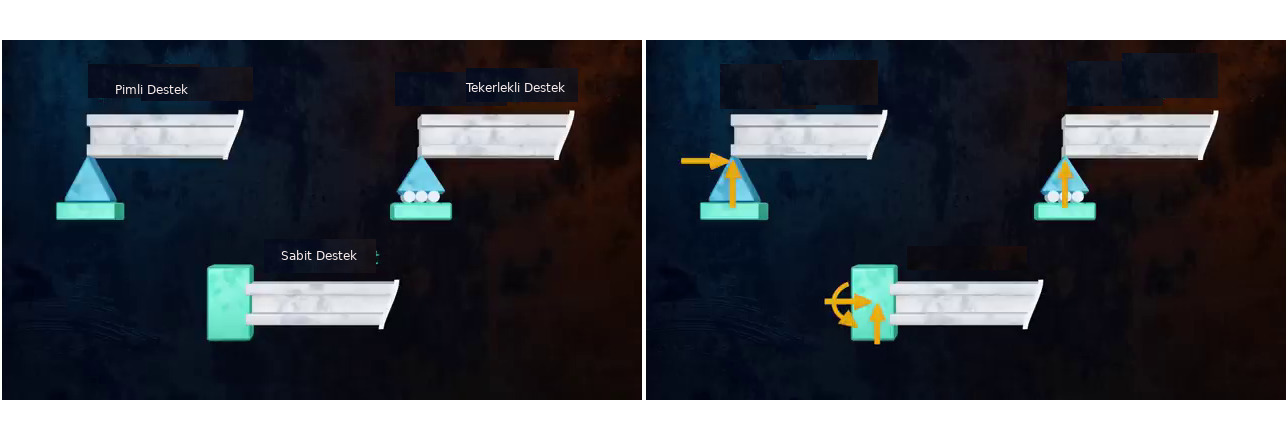
\includegraphics[width=25em]{phy_020_strs_01b_01.jpg}

Üstteki soldaki resimde mesela iki boyutta pimli destek dönüşe izin verir,
tekerlekli yatay sağ, sol hareketi ve dönüşü serbest bırakır. Sabit destekte hiç
harekete izin yoktur. Hangi harekete izin verilmediğine göre yük uygulanması
ardından üst sağdaki iç kuvvetler ortaya çıkacaktır, bunlar pimli durumda dikey
ve yatay kuvvetler, tekerlekli durumda dikey kuvvet, sabit durumda ise her üç
mümkün tepkilerdir, yani moment, dikey ve yatay.

Yükler noktasal ya da dağıtık şekilde uygulanabilir, altta noktasal kuvvet,
dağıtık kuvvet ve noktasal moment örneklerini görüyoruz.

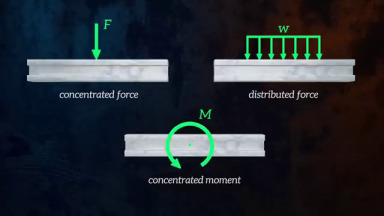
\includegraphics[width=20em]{phy_020_strs_01b_02.jpg}

Bir kirişin hissettiği içsel kuvvetler ve momentleri hesaplamak için denge
denklemleri kullanılır, bu denkleme (ve temel fiziğe göre) kırise uyguladığımız
hayali bir kesitte etki eden tüm kuvvetler ve momentler birbirini
dengelemelidir. Kesit tüm kiriş boyunca kaydırılır ve her noktadaki kuvvetler
hesaplanır.

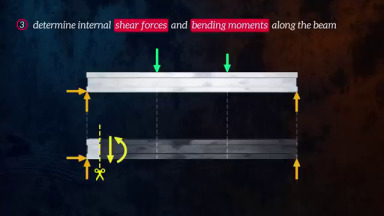
\includegraphics[width=20em]{phy_020_strs_01b_03.jpg}

Tipik olarak problemin beklediği kesim kuvveti ve bükülme momenti grafikleridir,
bu grafiklerde $x$ ekseni yatay olarak kirişın kendisi, $y$ ekseni ise o noktada
etki eden kesim ya da moment büyüklüğüdür. 

Problem 1














[devam edecek]

Kaynaklar 

[1] The Efficient Engineer, {\em Understanding Shear Force and Bending Moment Diagrams},
    \url{https://youtu.be/C-FEVzI8oe8}

\end{document}
